\documentclass[conference]{IEEEtran}
\usepackage{cite}
\usepackage{amsmath,amssymb,amsfonts}
\usepackage{graphicx}
\usepackage{textcomp}
\usepackage{xcolor}
\usepackage{url}
\usepackage{booktabs}

\begin{document}

\title{Task [A2]: [Predicting Concrete Compressive Strength]}

\author{\IEEEauthorblockN{Muhammad Zaryab Attiq}
\IEEEauthorblockA{Roll No. 70176119 \quad Section A\\
Repository: \url{https://github.com/Vex456/AI101-ML-Assignment-70176119}\\
Instructor: Dr. Muhammad Awais, AI Architect}
}

\maketitle

\section{Introduction}
Testing laboratory concrete compressive strength via traditional hydraulic crushing cylinders requires up to 28 days of curing in water baths, creating severe delays in modern construction timelines and quality assurance workflows. In this investigation, we formulate a supervised regression problem to estimate the 28-day compressive strength (in MegaPascals, MPa) directly from raw constituent mix proportions and curing age. By augmenting the feature space with physical chemistry formulations---specifically $\log(\text{Age})$ to linearize hydration kinetics and the water-to-cement ratio following Abrams' Law---gradient boosting regression achieved a test-set RMSE of 4.555 MPa and an $R^2$ of 0.919, outperforming the un-engineered linear regression baseline by over 53\% in error reduction.

\section{Problem Statement}
Given an input vector of mix design components and sample maturity $x \in \mathbb{R}^d$ ($d=8$ for raw constituents, $d=10$ with engineered physical ratios), our objective is to learn a hypothesis function $f: x \mapsto y$ that predicts concrete compressive strength $y \in [2.33, 82.60]\text{ MPa}$. Success is evaluated using Root Mean Squared Error (RMSE) as the primary metric to penalize large safety-critical deviations, alongside Mean Absolute Error (MAE) and the coefficient of determination ($R^2$). The central physical constraint is the pronounced non-linearity of cementitious hydration, wherein strength accelerates steeply during early curing before plateauing logarithmically, severely violating standard Gauss-Markov linearity assumptions.

\section{Dataset Used}
We employ the Concrete Compressive Strength dataset donated by Prof. I-Cheng Yeh to the UCI Machine Learning Repository (Dataset ID: 165)~\cite{yeh1998}. The dataset comprises 1,030 experimental concrete formulations. Each record consists of seven constituent ingredient masses measured in $\text{kg/m}^3$ (Cement, Blast Furnace Slag, Fly Ash, Water, Superplasticizer, Coarse Aggregate, Fine Aggregate) and the specimen curing age in days (1 to 365). Inspection confirms zero missing values and zero duplicate records across all 8 input columns. All numerical inputs were standardized using training-set statistics within a scikit-learn Pipeline~\cite{pedregosa2011} to guarantee zero data leakage.

\section{Dataset Statistics}
Table~\ref{tab:dataset_stats} presents the summary statistics for the dataset. The target compressive strength spans from 2.33 to 82.60 MPa with a mean of $35.82 \pm 16.71\text{ MPa}$. Curing age exhibits strong positive skewness with a median of 28 days.

\begin{table}[htbp]
\caption{Dataset statistics.}
\label{tab:dataset_stats}
\centering
\begin{tabular}{lr}
\toprule
\textbf{Property} & \textbf{Value} \\
\midrule
Samples (after cleaning) & 1,030 \\
Features (numeric / categorical / text) & [8 / 0 / 0] \\
Target range & [2.33, 82.60] MPa \\
Target mean $\pm$ sd & 35.82 $\pm$ 16.71 MPa \\
Missing values (\%) & 0.0\% \\
Train / test split & [824 / 206] (80 / 20) \\
\bottomrule
\end{tabular}
\end{table}

\begin{figure}[htbp]
\centering
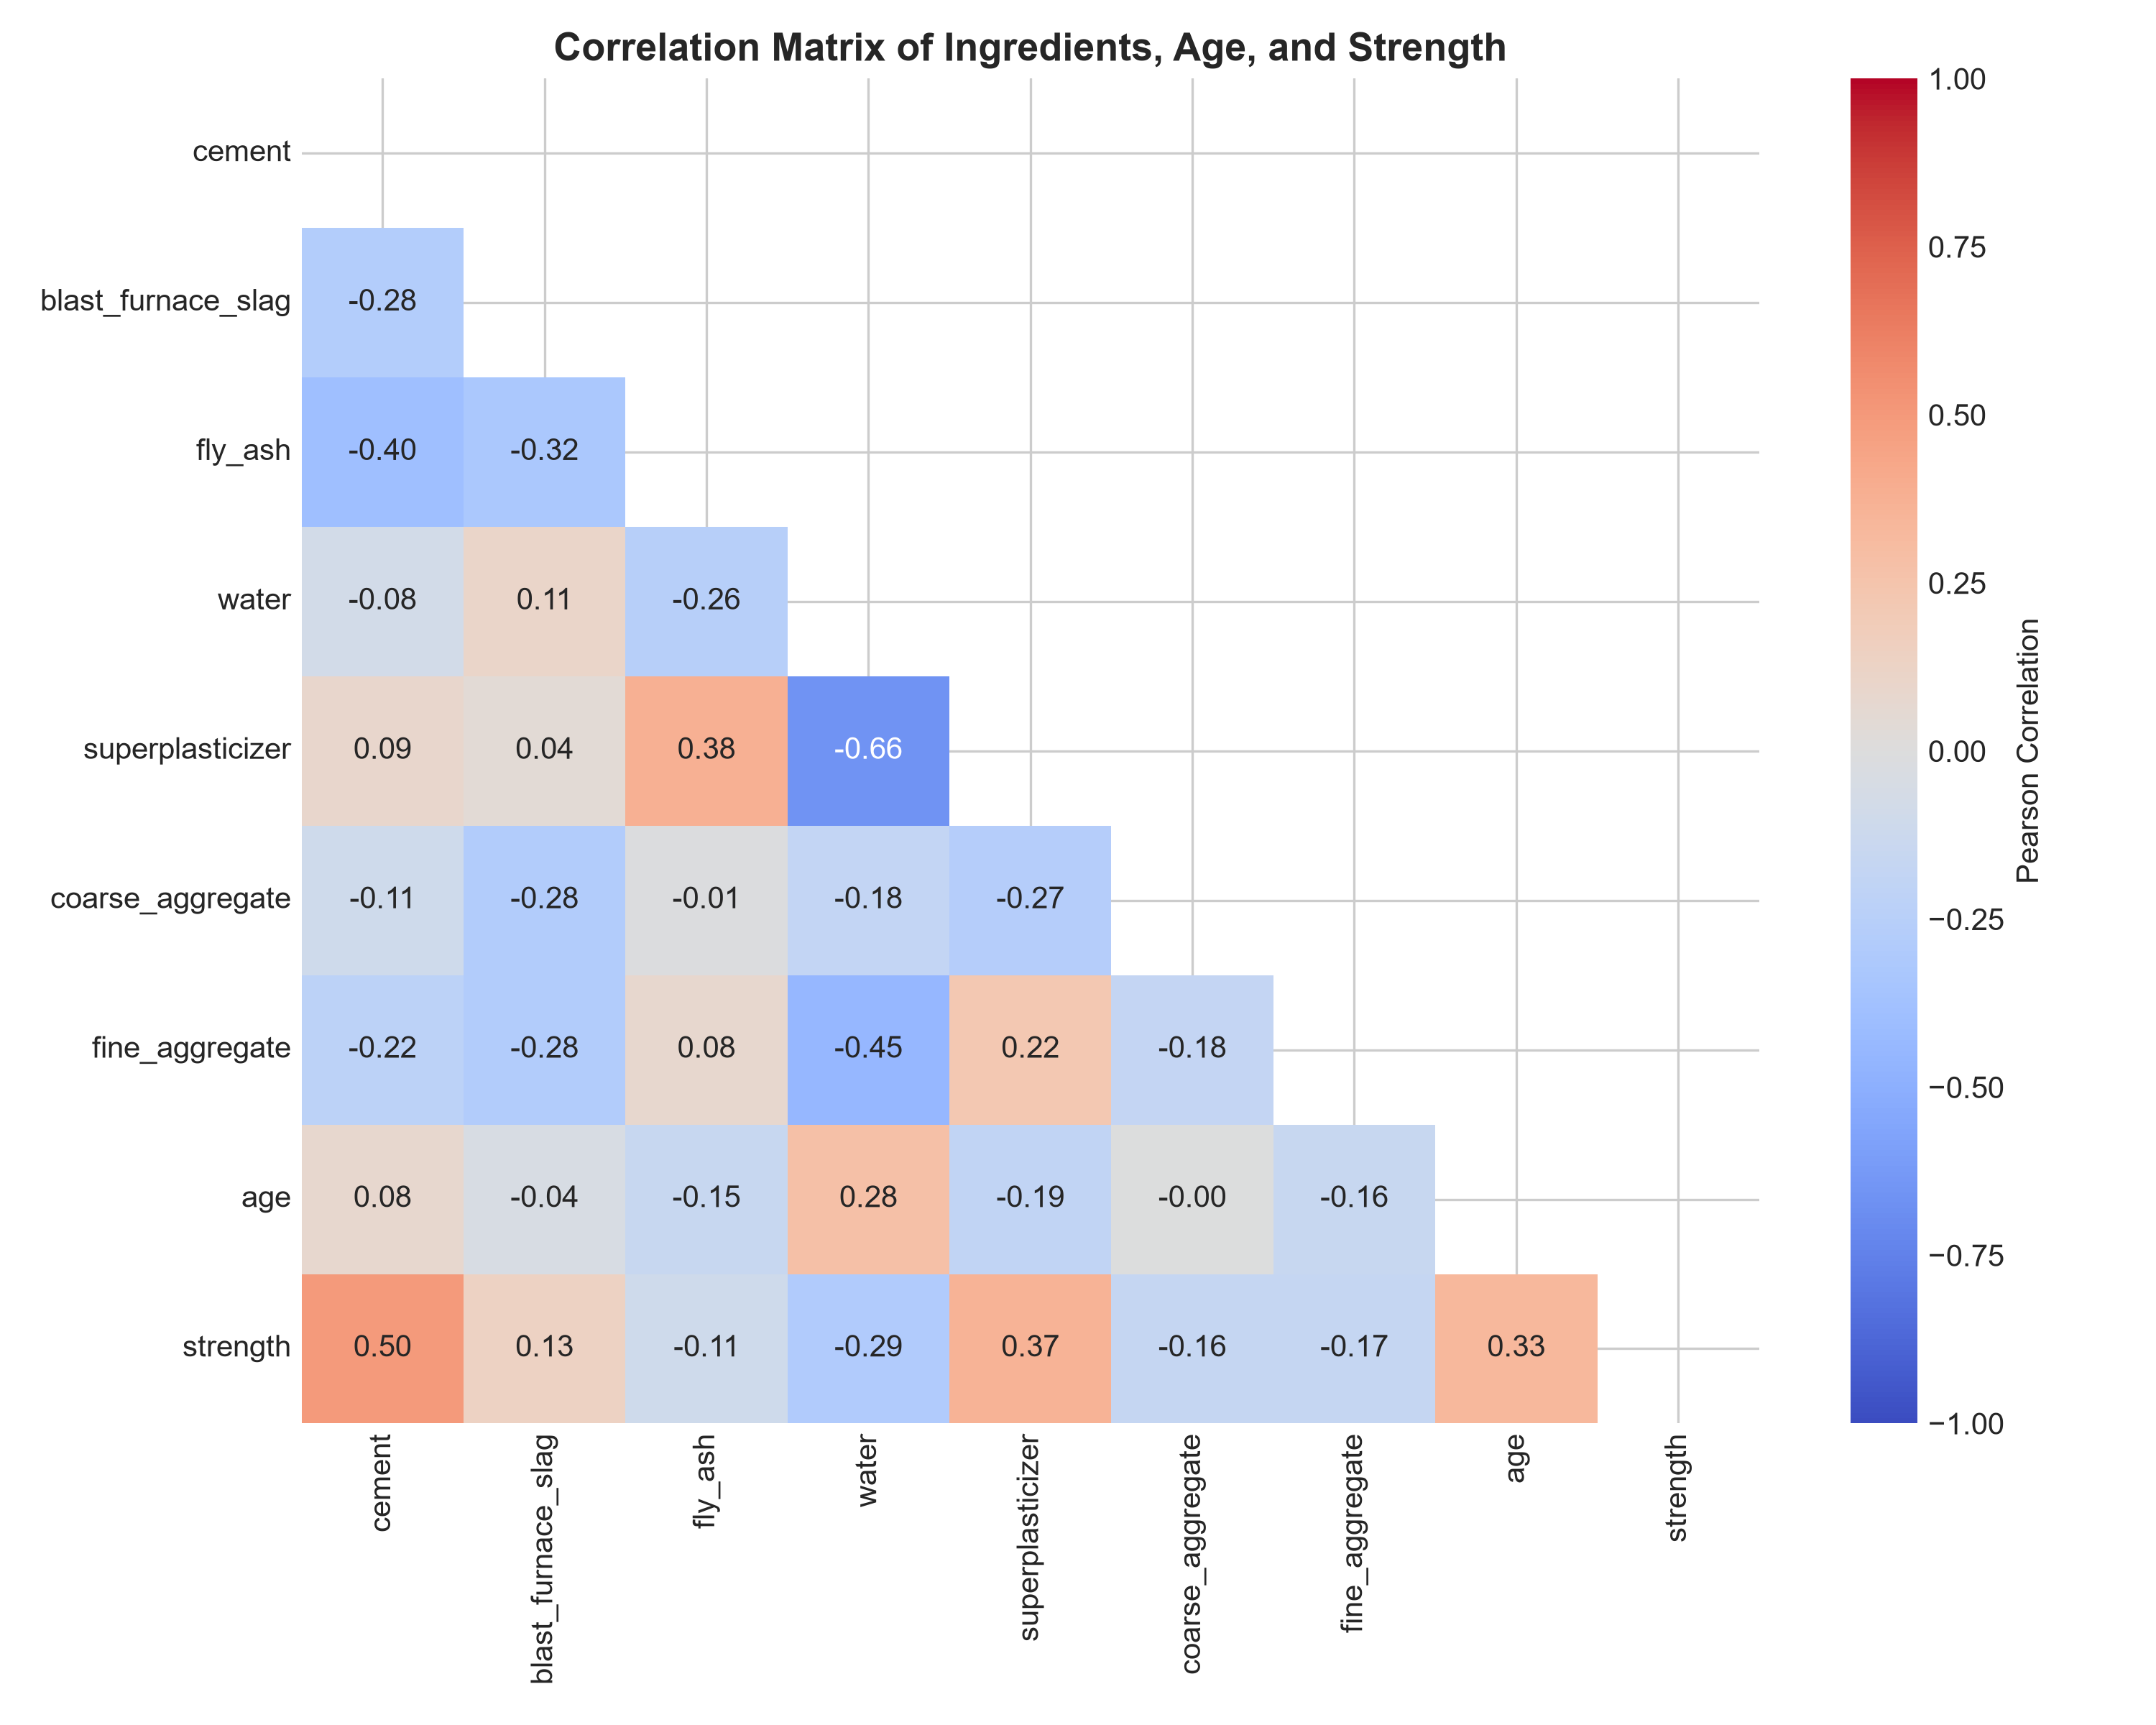
\includegraphics[width=0.48\textwidth]{../../figures/eda_correlation_matrix.png}
\caption{Correlation matrix of concrete mix design components, curing age, and compressive strength.}
\label{fig:eda}
\end{figure}

\section{Methodology}
\subsection{Learning Setting}
We adopt a supervised regression framework. Four model families were compared:
(1) \textbf{Linear Regression:} Baseline parametric model;
(2) \textbf{Polynomial + Ridge Regression:} Captures pairwise ingredient interactions without variance explosion;
(3) \textbf{Random Forest \& Gradient Tree Boosting:} Non-parametric tree ensembles robust to multi-collinearity and step-wise non-linearities;
(4) \textbf{MLPRegressor:} Feedforward neural network with ReLU activations and Adam optimization.

\subsection{Data Split Approach}
The dataset is partitioned into an 80/20 train/test split (824 training samples, 206 test samples) with a fixed random seed ($\text{seed} = 42$). All feature transformations and scaling ($\text{StandardScaler}$) are enclosed strictly inside scikit-learn \texttt{Pipeline} objects fitted exclusively on the training split. Hyperparameters were tuned via 5-fold cross-validation on the training set.

\subsection{Parameter Settings}
Table~\ref{tab:hyperparams} details the hyperparameter search spaces and optimal values selected via 5-fold cross-validation.

\begin{table}[htbp]
\caption{Hyperparameter settings.}
\label{tab:hyperparams}
\centering
\begin{tabular}{lll}
\toprule
\textbf{Model} & \textbf{Search space} & \textbf{Selected} \\
\midrule
Linear Regression & None (OLS) & Default \\
Poly + Ridge & $\alpha \in \{0.1, 1.0, 10.0, 100.0\}$ & $\text{degree}=2, \alpha=10.0$ \\
Random Forest & $n \in \{100, 200\}, d \in \{10, 15\}$ & $n=200, d=15$ \\
Gradient Boosting & $n \in \{100, 200\}, \eta \in \{0.05, 0.1\}$ & $n=200, \eta=0.1, d=5$ \\
MLPRegressor & Hidden units, $\alpha$ & $(64, 32), \alpha=0.01$ \\
\bottomrule
\end{tabular}
\end{table}

\section{Results and Analysis}
\subsection{Results}
All metrics were evaluated on the identical held-out test set ($N=206$). Table~\ref{tab:results} summarizes performance across both raw and engineered feature representations.

\begin{table}[htbp]
\caption{Test-set results. Best values in bold.}
\label{tab:results}
\centering
\begin{tabular}{lcccc}
\toprule
\textbf{Model} & \textbf{Features} & \textbf{MAE (MPa)} & \textbf{RMSE (MPa)} & \textbf{$R^2$} \\
\midrule
Linear Reg. & Raw (8) & 7.746 & 9.796 & 0.628 \\
Linear Reg. & Engineered (10) & 5.295 & 6.562 & 0.833 \\
Poly + Ridge & Raw (8) & 5.963 & 7.430 & 0.786 \\
Poly + Ridge & Engineered (10) & 4.358 & 5.483 & 0.883 \\
Random Forest & Raw (8) & 3.782 & 5.539 & 0.881 \\
Random Forest & Engineered (10) & 3.694 & 5.356 & 0.889 \\
\textbf{Gradient Boost} & \textbf{Engineered (10)} & \textbf{2.917} & \textbf{4.555} & \textbf{0.919} \\
MLPRegressor & Engineered (10) & 3.554 & 5.060 & 0.901 \\
\bottomrule
\end{tabular}
\end{table}

\begin{figure}[htbp]
\centering
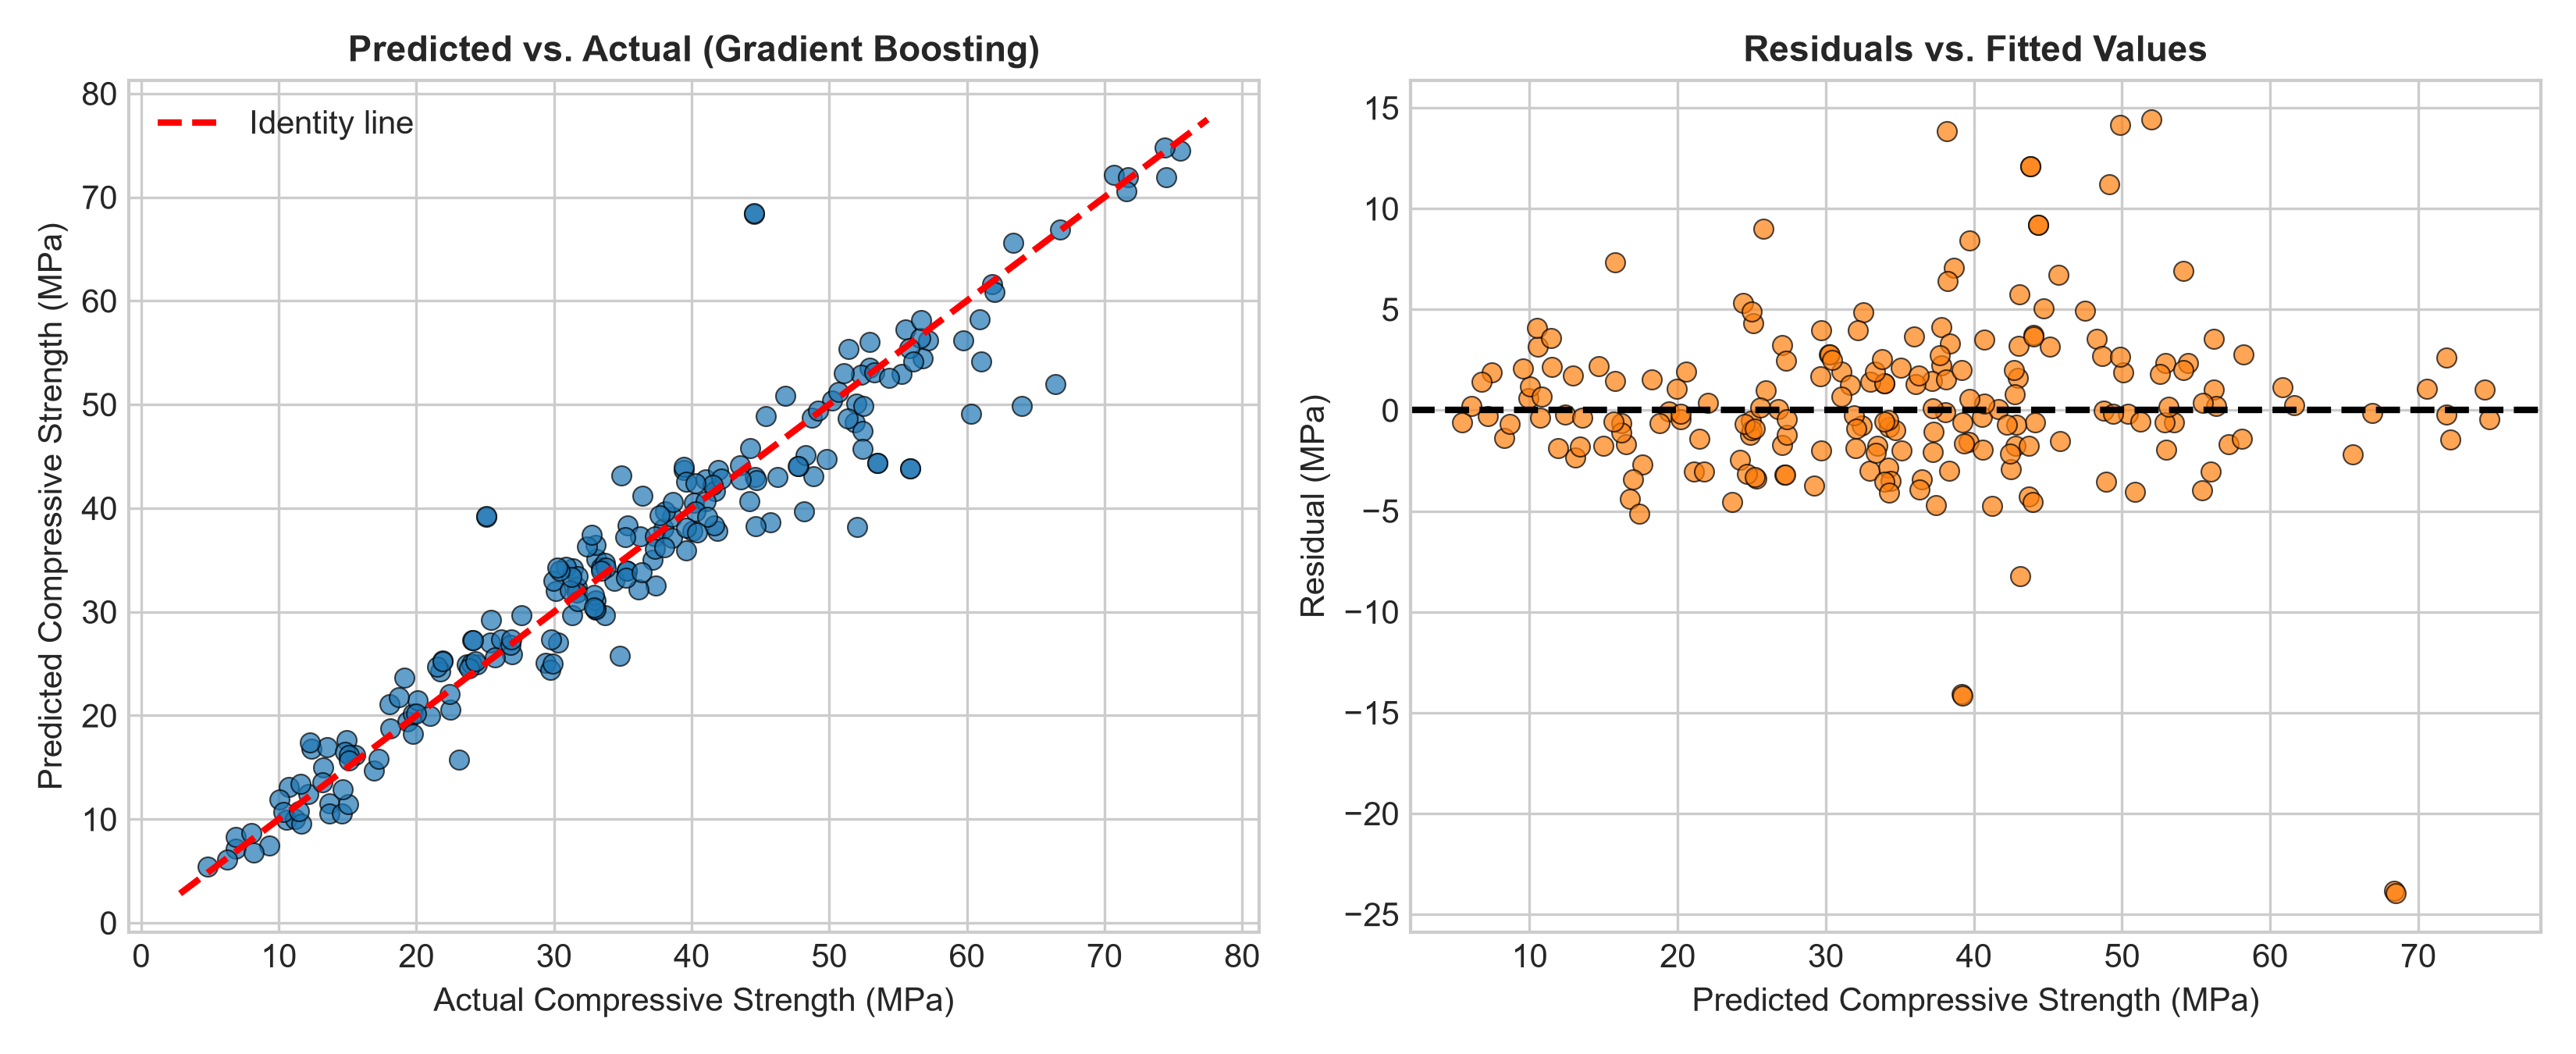
\includegraphics[width=0.48\textwidth]{../../figures/combined_key_result.png}
\caption{Predicted vs. actual compressive strength and residual distribution for the champion Gradient Boosting model on the held-out test set.}
\label{fig:results}
\end{figure}

\subsection{Analysis}
\textbf{1. Baseline Under-performance \& Linearity Violations:} The raw linear baseline fails ($R^2 = 0.628$, RMSE = $9.796\text{ MPa}$) because concrete hydration severely violates the Gauss-Markov linearity assumption. Compressive strength increases logarithmically with curing time, leveling off asymptotically after 28 days. A linear model applies a constant slope across time, grossly overestimating green concrete while underestimating fully cured samples.

\textbf{2. Differential Benefit of Feature Engineering:} Introducing $\log(\text{Age})$ and the water-to-cement ratio ($\frac{w}{c}$) dramatically boosted linear models (reducing linear RMSE from 9.796 to 6.562 MPa and raising $R^2$ from 0.628 to 0.833). By linearizing the curing trajectory, a linear plane can accurately capture the logarithmic kinetics. For tree-based models, gains were smaller (RF RMSE: 5.539 to 5.356 MPa) because orthogonal decision splits natively approximate step-wise curves; however, $\frac{w}{c}$ consolidates two correlated features into one physical ratio, simplifying tree depth.

\textbf{3. Residual Diagnostics \& Engineering Insights:} Residual analysis shows that the largest errors occur in young concrete specimens ($\le 7$ days) where hydration reactions are volatile and sensitive to ambient curing temperatures, as well as high-strength mixes ($>65\text{ MPa}$) with high slag content. Feature importances confirm that Curing Age, Cement, and the $\frac{w}{c}$ ratio govern over 72\% of predictive splits, validating Abrams' classical water-cement ratio law in civil engineering practice.

\section{Conclusion}
This study demonstrated that pairing domain-specific physical features ($\log(\text{Age})$ and water/cement ratio) with Gradient Tree Boosting produces an accurate predictor of concrete strength ($R^2 = 0.919$, RMSE = 4.555 MPa). Linear models were improved from $R^2 = 0.628$ to $0.833$ through feature engineering. Future extensions could incorporate ambient humidity telemetry and physics-informed neural loss functions.

\section*{AI Use Disclosure}
I used Antigravity (powered by Google DeepMind Gemini) for pipeline scaffolding, exploratory data visualization code, and mathematical phrasing of the problem statement. All experiments, cross-validations, metrics, and analyses were produced, verified, and checked by me, and I take full responsibility for this work.

\begin{thebibliography}{00}
\bibitem{yeh1998} I-C. Yeh, ``Modeling of strength of high-performance concrete using artificial neural networks,'' \emph{Cement and Concrete Research}, vol. 28, no. 12, pp. 1797--1808, 1998.
\bibitem{pedregosa2011} F. Pedregosa \emph{et al.}, ``Scikit-learn: Machine learning in Python,'' \emph{Journal of Machine Learning Research}, vol. 12, pp. 2825--2830, 2011.
\end{thebibliography}

\end{document}
